\documentclass[a4paper,oneside,12pt]{extarticle}

\usepackage[utf8]{inputenc}
\usepackage[english]{babel}
\usepackage{amssymb}
\usepackage{amsthm}
\usepackage{enumitem}
\usepackage{geometry}
\usepackage{mathtools}
\usepackage{hyperref}
\usepackage{tikz}
\usepackage{pgfplots}
\pgfplotsset{compat=1.18}
\usetikzlibrary{decorations.pathreplacing,arrows.meta}

\geometry
{
lmargin=15mm,
rmargin=15mm,
tmargin=10mm,
bmargin=10mm,
includeheadfoot
}
\pagestyle{empty}
\frenchspacing


\theoremstyle{plain}
\newtheorem{proposition}{Proposition}
\newtheorem{lemma}[proposition]{Lemma}

\theoremstyle{definition}
\newtheorem{definition}[proposition]{Definition}
\newtheorem{example}[proposition]{Example}

\theoremstyle{remark}
\newtheorem{remark}[proposition]{Remark}


\newcommand*{\ges}{\geqslant}
\newcommand*{\les}{\leqslant}
\newcommand*{\ve}{\varepsilon}
\newcommand*{\E}{\mathbb{E}}
\newcommand*{\diag}{\textrm{diag}}
\newcommand*{\vf}{\varphi}
\newcommand*{\mbR}{\mathbb{R}}
\newcommand*{\mP}{\mathbb{P}}
\newcommand*{\mF}{\mathcal{F}}

\DeclarePairedDelimiter{\abs}{\lvert}{\rvert}


\begin{document}

%--------------------------------------------------------------------
\begin{center}
{\LARGE\bfseries Cohort Component Models:\\[5pt]
Time-Series Structure and Forecast Foundations}

\bigskip
{\large Boris Garbuzov}

\bigskip
{\small April 2026}
\end{center}

\bigskip
\tableofcontents
\bigskip

%--------------------------------------------------------------------
\section{Introduction}
%--------------------------------------------------------------------

At work I have been forecasting workforce volume by standard methods like
ARIMA and neural nets. Then I came across the cohort component
method---apparently the standard tool for demographic contexts, and
something I had never encountered in school. I had to figure out from
scratch how to measure stock, inflow, and outflow, and compare it to other
approaches. It turned out to be structurally a generalisation of AR(1).

Along the way I wanted to refresh the basics: what does a forecast problem
actually look like at the level of definitions, what is the difference
between a predictor and an estimator, where does the irreducible error floor
come from. And a further question: when we draw a forecast curve, I wanted
to visually combine it with the full underlying process---a partial
reconstruction of the bundle of sample paths. That connects prediction with
statistical inference in a way I had not thought about carefully before.

I moved on from this topic and did not want to lose what I had accumulated.
So I put it all together here. It is an eclectic piece. No claims to new
results or business insights. But if you have worked on similar
problems---workforce planning, membership registries, any population with
inflow and attrition---maybe we are on the same wavelength.

\medskip\noindent
The note is structured as follows. Section~\ref{sec:snapshots} builds the
cohort component model as a set-theoretic accounting identity.
Section~\ref{sec:settheory} gives canonical definitions of inflow and
outflow. Section~\ref{sec:ar1} shows that under constant rates the
recursion is exactly AR(1) with drift, and the multi-group version is
VAR(1). Section~\ref{sec:curvefitting} covers estimation of age profiles.
Section~\ref{sec:forecast} develops the statistical foundation of point
forecasting in the i.i.d.\ setting. Section~\ref{sec:inference_vs_prediction}
examines what it means to attach a bundle of sample paths to a forecast
curve, using AR(1) as the concrete example.


%--------------------------------------------------------------------
\section{Cohort Snapshots and the Accounting Identity}
\label{sec:snapshots}
%--------------------------------------------------------------------

\subsection{Notation: beginning versus end of period}

Let $S_t^b$ and $S_t^e$ denote the set of cohort members present at the
beginning and end of time period $t$ respectively. In general
$S_{t+1}^b \neq S_t^e$, and so $\abs{S_{t+1}^b} \neq \abs{S_t^e}$.

\begin{example}
Suppose members $\{X,Y,Z\}$ are present during period $t$. At the end of
$t$, member $Z$ exits; at the start of $t+1$, members $U$ and $V$ enter.
Then
\[
S_t^b = S_t^e = \{X,Y,Z\}, \qquad
S_{t+1}^b = \{X,Y,U,V\}.
\]
The discrepancy between $S_t^e$ and $S_{t+1}^b$ reflects the simultaneous
exit of $Z$ and entry of $U,V$ at the period boundary.
\end{example}

\begin{example}
Suppose $\{X,Y,Z\}$ are present at the start of $t$, member $U$ enters
during $t$, member $V$ enters at the start of $t+1$, and all five members
remain through $t+1$. Then
\[
S_t^b = \{X,Y,Z\},\quad
S_t^e = \{X,Y,Z,U\},\quad
S_{t+1}^b = \{X,Y,Z,U,V\}.
\]
\end{example}

The choice of whether recorded data represents the cohort at the beginning
or end of each period is a modelling decision that affects all subsequent
recursions.

\subsection{Time-series recursion: beginning-of-period convention}

Let $I_t$ denote the set of members who enter during period $t$ and $O_t$
the set who exit. The general recursion is
\begin{equation}
\label{eq:main_equation_1}
\abs{S_{t+1}^b} = \abs{S_t^b} + \abs{I_t} - \abs{O_t}.
\end{equation}
Define the attrition rate $r_t = \abs{O_t}/\abs{S_t^b}$. When the
probability of exiting in the same period as entry is negligible, outflow
draws only from the beginning-of-period stock, giving
\begin{equation}
\label{eq:main_equation_2}
\abs{S_{t+1}^b} = (1-r_t)\abs{S_t^b} + \abs{I_t}.
\end{equation}

\subsection{Time-series recursion: end-of-period convention}

Under the end-of-period convention,
\begin{equation}
\label{eq:main_equation_3}
\abs{S_{t+1}^e} = \abs{S_t^e} + \abs{I_{t+1}} - \abs{O_{t+1}},
\end{equation}
with attrition rate $r_t = \abs{O_t}/\abs{S_{t-1}^e}$, leading to
\begin{equation}
\label{eq:main_equation_4}
\abs{S_t^e} = (1-r_t)\abs{S_{t-1}^e} + \abs{I_t}.
\end{equation}

Both recursions have the same algebraic structure; only the index
convention differs. In what follows we adopt the end-of-period convention
and write $S_t$ for $\abs{S_t^e}$, dropping the superscript.

\subsection{Example}

Consider the following sequence of events:
\begin{itemize}
\item on day 1 of month $A$, the cohort consists of $\{X,Y,Z\}$;
\item on day 2, $Z$ exits and $U$ enters;
\item on the last day, $Y$ exits and $V$ enters;
\item on day 1 of month $B$, $X$ exits and $W$ enters.
\end{itemize}
Then:
\[
S_A^b = \{X,Y,Z\},\quad S_A^e = \{X,U,V\},\quad
I_A = \{U,V\},\quad O_A = \{Y,Z\},
\]
and $W \in I_B$, $X \in O_B$.


%--------------------------------------------------------------------
\section{Set-Theoretic Foundations}
\label{sec:settheory}
%--------------------------------------------------------------------

\subsection{Canonical definitions}

\begin{definition}
Let $S_t$ be the set of cohort members at the end of period $t$. Define
\[
I_t = S_t \setminus S_{t-1} \quad\text{(inflow)}, \qquad
O_t = S_{t-1} \setminus S_t \quad\text{(outflow)}.
\]
\end{definition}

From these definitions: $O_t \subset S_{t-1}$ so $\abs{O_t} \les \abs{S_{t-1}}$;
$I_t \subset S_t$ so $\abs{I_t} \les \abs{S_t}$. The pairs
$(I_t, O_t)$, $(S_t, I_{t+1})$, $(S_t, O_t)$, and $(I_t, S_{t-1}\cap S_t)$
are all disjoint.

\begin{remark}
A member who enters and exits within the same period appears in neither
$I_t$ nor $O_t$, since they are absent from both $S_t$ and $S_{t-1}$.
A member who enters at the very end of $t-1$ (appearing in $S_{t-1}$) but
exits at the start of $t$ (absent from $S_t$) is counted in $I_{t-1}$ and
$O_t$, even if their effective tenure was shorter than that of the first
member. This boundary effect is an inherent feature of the snapshot
convention.
\end{remark}

\subsection{The accounting identity}

\begin{proposition}
\label{prop:identity}
For all $t \ges 1$,
\begin{equation}
\label{eq:main_equation}
\abs{S_{t+1}} = \abs{S_t} - \abs{O_{t+1}} + \abs{I_{t+1}}.
\end{equation}
\end{proposition}

\begin{proof}
From the definitions, $S_{t+1} = (S_t \setminus O_{t+1}) \cup I_{t+1}$
with the two sets on the right disjoint. Since $O_{t+1} \subset S_t$,
we have $\abs{S_t \setminus O_{t+1}} = \abs{S_t} - \abs{O_{t+1}}$,
and the result follows.
\end{proof}

\subsection{Outflow and inflow rates}

Writing $S(t)$, $O(t)$, $I(t)$ for the cardinalities, equation
\eqref{eq:main_equation} becomes
\begin{equation}
\label{eq:time_series}
S(t+1) = S(t) - O(t+1) + I(t+1).
\end{equation}
Define the rates
\begin{align}
r_t^O &= \frac{O(t+1)}{S(t)}, \label{eq:outflow_rate}\\[3pt]
r_t^I &= \frac{I(t+1)}{S(t)}, \label{eq:inflow_rate_1}\\[3pt]
R_t^I &= \frac{I(t)}{S(t)}. \label{eq:inflow_rate_2}
\end{align}
Since $O(t+1) \les S(t)$, we have $r_t^O \in [0,1]$. The rate $r_t^I$
may exceed $1$ if inflow is large; $R_t^I \in [0,1]$ since $I_t \subset S_t$.


%--------------------------------------------------------------------
\section{AR(1) and VAR(1) Representations}
\label{sec:ar1}
%--------------------------------------------------------------------

\subsection{VAR(1) structure of the scalar model}

Define the state vector $X(t) = (S(t), O(t+1), I(t+1))^\top$ and write
the VAR(1) model $X(t+1) = c + AX(t) + e(t+1)$. In expanded form:
\[
\begin{cases}
S(t+1) = c_1 + A_{11}S(t) + A_{12}O(t+1) + A_{13}I(t+1) + e_1(t+1),\\
O(t+2) = c_2 + A_{21}S(t) + A_{22}O(t+1) + A_{23}I(t+1) + e_2(t+1),\\
I(t+2) = c_3 + A_{31}S(t) + A_{32}O(t+1) + A_{33}I(t+1) + e_3(t+1).
\end{cases}
\]
Comparing the first equation with \eqref{eq:time_series} gives
$c_1 = 0$, $A_{11} = 1$, $A_{12} = -1$, $A_{13} = 1$.
If the rates $r^O$ and $R^I$ are constant, then
$O(t+2) = r^O S(t+1)$ and $I(t+2) = R^I S(t+1)$, so the second and
third equations are proportional to the first.

\subsection{AR(1) with drift}

Under constant attrition rate $r^O$ and constant inflow $I$, adding a
mean-zero noise term $\ve(t)$, equation \eqref{eq:time_series} becomes
\begin{equation}
\label{eq:ar1_drift}
S(t) = (1-r^O)\cdot S(t-1) + I + \ve(t).
\end{equation}
This is an AR(1) process with drift. The coefficient $1-r^O \in (0,1)$
guarantees stationarity of the noise component.

\subsection{Long-run equilibrium}

Taking expectations with $m(t) = \E S(t)$:
\[
m(t) = (1-r^O)\cdot m(t-1) + I.
\]
Iterating and summing the geometric series,
\[
m(t) = (1-r^O)^t\cdot m(0) + \frac{1-(1-r^O)^t}{r^O}\cdot I.
\]
As $t \to \infty$, $(1-r^O)^t \to 0$ and
\[
m(t) \;\to\; \frac{I}{r^O}.
\]
The long-run cohort size is determined entirely by the ratio of inflow to
attrition rate.

\subsection{Stationary decomposition}

Setting $S_0(t) = S(t) - m(t)$, the centred process satisfies
\[
S_0(t) = (1-r^O)\cdot S_0(t-1) + \ve(t),
\]
which is a zero-mean AR(1). Since $r^O \in (0,1)$, this process is
stationary. The original series decomposes as $S(t) = S_0(t) + m(t)$,
where the first component fluctuates around zero and the second converges
to $I/r^O$.

\subsection{Multi-age-group VAR(1)}

Let $S_i(t)$ be the cohort size in age group $i = 1,\ldots,N$, with
constant age-specific inflows $I_i$ and attrition rates $r_i^O$. The
system
\[
\begin{cases}
S_1(t) = I_1 + \ve_1(t),\\
S_i(t) = (1-r_{i-1}^O)\cdot S_{i-1}(t-1) + I_i + \ve_i(t),
  \quad i = 2,\ldots,N,
\end{cases}
\]
can be written as $X(t) = AX(t-1) + I + \ve(t)$, where
$X(t) = (S_1(t),\ldots,S_N(t))^\top$ and
\[
A =
\begin{pmatrix}
0 & 0 & \cdots & 0\\
1-r_1^O & 0 & \cdots & 0\\
0 & 1-r_2^O & \cdots & 0\\
\vdots & \vdots & \ddots & \vdots\\
0 & 0 & \cdots\; 1-r_{N-1}^O & 0
\end{pmatrix}.
\]
This is a VAR(1) model. The matrix $A$ is strictly sub-diagonal with
non-negative entries; its spectral radius satisfies $\rho(A) < 1$,
guaranteeing stability.

\begin{remark}
If age groups span more than one year, each time unit must equal the
group width.
\end{remark}


%--------------------------------------------------------------------
\section{Connection between AR(1) with and without Drift}
\label{sec:ar1_drift}
%--------------------------------------------------------------------

\begin{proposition}
\label{prop:explicit_formula}
Let $x_n = \vf x_{n-1} + \ve_n$, $n \ges 1$, with $x_0$ given and
$\vf \in \mbR$. Then
\[
x_n = \vf^n x_0 + \sum_{i=1}^n \vf^{n-i}\ve_i, \qquad n \ges 0.
\]
\end{proposition}

\begin{proof}
By induction: the formula holds for $n=0,1$. If it holds for $n$, then
\[
x_{n+1} = \vf x_n + \ve_{n+1}
= \vf^{n+1}x_0 + \sum_{i=1}^n \vf^{n+1-i}\ve_i + \ve_{n+1}
= \vf^{n+1}x_0 + \sum_{i=1}^{n+1} \vf^{n+1-i}\ve_i. \qedhere
\]
\end{proof}

\begin{proposition}
\label{prop:decomposition}
Let $y_n = \vf y_{n-1} + \delta + \ve_n$, where $\vf,\delta\in\mbR$,
$\{\ve_n\}$ are i.i.d.\ with zero mean, and $y_0$ has finite mean.
Then $y_n = x_n + m_n$, where
\[
x_n = \vf x_{n-1} + \ve_n \quad\text{(zero-mean AR(1))}, \qquad
m_n = \vf m_{n-1} + \delta \quad\text{(deterministic)}.
\]
\end{proposition}

\begin{proof}
Set $m_n = \E y_n$. Taking expectations in the recursion gives
$m_n = \vf m_{n-1} + \delta$. Then $x_n = y_n - m_n$ satisfies
$x_n = \vf x_{n-1} + \ve_n$.
\end{proof}

\begin{proposition}
For any $n \ges 0$,
\[
y_n = \vf^n x_0 + \sum_{i=1}^n \vf^{n-i}\ve_i
      + \vf^n m_0 + \frac{1-\vf^n}{1-\vf}\,\delta
\qquad (\vf \neq 1).
\]
\end{proposition}

\begin{proof}
Apply Proposition~\ref{prop:explicit_formula} to both $x_n$ and $m_n$,
then use the decomposition $y_n = x_n + m_n$.
\end{proof}

When $\ve_i \equiv 0$, the deterministic trajectory takes the compact form
\begin{equation}
\label{eq:y_sequence_a_b_def}
y_n = a + b\vf^n, \qquad
a = x_0 + m_0 - \frac{\delta}{1-\vf}, \quad
b = \frac{\delta}{1-\vf} \qquad (\vf \neq 1).
\end{equation}
For $\vf = 1$ the formula is replaced by $y_n = x_0 + m_0 + n\delta$.


%--------------------------------------------------------------------
\section{Auxiliary: Estimating Age Profiles from Cohort Data}
\label{sec:curvefitting}
%--------------------------------------------------------------------

The AR(1) and VAR(1) models require numerical values for $r^O$ and $I$.
These must be estimated from historical data. This section describes the
estimation problem that arises when the data take the form of annual
cohort bar charts indexed by age.

\subsection{Empirical age profiles}

For each annual cohort $i = 1,\ldots,n$, two age profiles are of interest:
\begin{itemize}
\item the \emph{inflow count profile}: for each age $a$, the number of
  members $I_i(a)$ who entered at age $a$;
\item the \emph{outflow rate profile}: for each age $a$, the ratio
  $r_i^O(a) = O_i(a)/S_i(a)$.
\end{itemize}
Plotting these as bar charts---age on the horizontal axis, the respective
quantity on the vertical---gives the raw empirical picture.

Such bar charts are typically irregular for two reasons. First,
\emph{gaps}: not every age is represented in every cohort, especially at
the extremes where cohort sizes are small. Second, \emph{noise}: the ratio
$O_i(a)/S_i(a)$ is volatile when $S_i(a)$ is small, producing
bar-to-bar fluctuations even if the underlying rate is smooth.
Naively averaging across cohorts propagates both defects.

\subsection{Two objectives of curve fitting}

Fitting a parametric curve $f(a;\theta)$ to the bar charts serves two
distinct purposes that should be kept separate.

The first is \emph{smoothing}: replacing noisy, gappy bars with a
continuous curve that can be evaluated at any age, interpolating over
missing values and suppressing sampling noise.

The second is \emph{structural modelling}: imposing a functional form that
encodes a substantive hypothesis about how the rate or count varies with
age. For example:
\begin{itemize}
\item an \emph{exponentially increasing} outflow rate,
  $f(a;\theta) = \theta_1 e^{\theta_2 a}$ with $\theta_2 > 0$, captures
  the hypothesis that exit risk grows proportionally with age;
\item a \emph{power-decay} form, $f(a;\theta) = \theta_1/(a-\theta_2)^{\theta_3}$
  with $\theta_3 \in (0,1)$, models a profile that is steep at low ages
  and has a heavy tail;
\item a \emph{hump-shaped} form (log-normal or log-logistic in $a$) models
  an inflow profile that peaks at a modal entry age and tapers on both sides.
\end{itemize}
The choice of family is a modelling decision: the parameters carry an
interpretation, and the choice should be guided both by the shape of the
empirical bar charts and by domain knowledge about the cohort dynamics.

\subsection{Multi-cohort least-squares estimation}

Pooling across all $n$ annual cohorts under the stationarity assumption
that $f(a;\theta)$ is stable over calendar time, the data are
\[
\{(a_{ij},\, y_{ij}),\; j = 1,\ldots,m_i\},\qquad i = 1,\ldots,n,
\]
where $a_{ij}$ is age and $y_{ij}$ the observed rate or count. Estimate
$\theta$ by minimising
\[
\mathrm{SSE}(\theta)
= \sum_{i=1}^n \sum_{j=1}^{m_i}
  \bigl(f(a_{ij};\theta) - y_{ij}\bigr)^2.
\]

\begin{remark}
Pooling under a common $\theta$ assumes the age profile is stable across
calendar years. Cohort-to-cohort variation visible in the bar charts is
evidence against this assumption and warrants further investigation.
\end{remark}

\subsection{Integrability constraint}

When $f(a;\theta)$ models a rate, the implied total probability of the
event occurring over all ages must not exceed one:
\[
\sum_{k=1}^{\infty} f(k;\theta) \les 1.
\]
This yields the constrained problem
\[
\begin{cases}
\displaystyle\sum_{i=1}^n \sum_{j=1}^{m_i}
  \bigl(f(a_{ij};\theta) - y_{ij}\bigr)^2 \mapsto \min,\\[6pt]
\displaystyle\sum_{k=1}^{\infty} f(k;\theta) \les 1,
\end{cases}
\]
handled by Lagrange multipliers with the infinite sum replaced by a
finite truncation.


%--------------------------------------------------------------------
\section{Forecast Foundations: Prediction without a Time Index}
\label{sec:forecast}
%--------------------------------------------------------------------

Before applying the AR(1) model to produce forecasts, it is worth
establishing what ``predicting a future observation'' means rigorously in
the simplest setting: an i.i.d.\ sequence, no time structure, no
covariates.

\subsection{Statistics, estimators, and predictors}

Fix a probability space $(\Omega,\mF,\mP)$ and let $Y_1,\ldots,Y_n$ be
random variables on it. A \emph{statistic} is any Borel-measurable
function $T = f(Y_1,\ldots,Y_n)$. Estimators and predictors are both
statistics; what distinguishes them is the nature of their target.

A \emph{point estimator} targets a non-random functional of the unknown
measure $\mP$, such as $\E_\mP Y$ or $\mathrm{Var}_\mP(Y)$.

A \emph{point predictor} targets a future, as yet unobserved random
variable $Y_{n+1}$. The target is random rather than fixed, and this
leads to different performance metrics: estimator quality is measured
relative to a fixed number, predictor quality relative to a random outcome.

Despite this difference, we will see that in the i.i.d.\ case, and
specifically under the squared-error criterion with target functional
$\theta(\mP) = \E_\mP Y$, the best predictor of $Y_{n+1}$ and the best
estimator of $\E Y$ are the same statistic. The two minimum values are
however different, and their gap has a precise meaning established below.

\subsection{The MSE criterion for constant predictors}

We measure the quality of a candidate constant predictor $c \in \mbR$ by
its \emph{mean squared error}
\[
\mathrm{MSE}(c) = \E(Y - c)^2.
\]

\begin{proposition}
\label{prop:best_constant}
Among all constants $c \in \mbR$, the MSE is minimised by $c^* = \E Y$,
and the minimum value is $\mathrm{Var}(Y)$.
\end{proposition}

\begin{proof}
$\E(Y-c)^2
= \mathrm{Var}(Y)
  - 2(c-\E Y)\underbrace{\E(Y-\E Y)}_{=\,0}
  + (c-\E Y)^2
= \mathrm{Var}(Y) + (c-\E Y)^2$,
minimised at $c^* = \E Y$.
\end{proof}

Extending to all measurable functions of $(Y_1,\ldots,Y_n)$ does not help:
since $Y_{n+1}$ is independent of the sample, the conditional expectation
$\E[Y_{n+1} \mid Y_1,\ldots,Y_n] = \E Y$ is still a constant. The
problem shifts from finding the optimal functional form to estimating
the unknown $\E_\mP Y$ from data.

\subsection{Two MSE criteria for sample-based statistics}

Suppose we observe $(Y_1,\ldots,Y_n)$ and wish to predict $Y_{n+1}$.
For any statistic $f(Y_1,\ldots,Y_n)$, define
\[
\mathrm{MSE}_{\mathrm{pred}}(f)
= \E\bigl(Y_{n+1} - f(Y_1,\ldots,Y_n)\bigr)^2,
\]
\[
\mathrm{MSE}_{\mathrm{est}}(f)
= \E\bigl(\E Y - f(Y_1,\ldots,Y_n)\bigr)^2.
\]
These are different quantities in general; however, the statistic
minimising one also minimises the other, though the two minimal values
differ. The exact relationship is established in
Proposition~\ref{prop:decomp}.

\subsection{The permutation lemma}

\begin{lemma}[Permutation equality]
\label{lem:permutation}
Let $Y_1,\ldots,Y_n,Y_{n+1}$ be i.i.d.\ with $\E Y_1^2 < \infty$, and
let $f:\mbR^n\to\mbR$ be Borel-measurable. Then
\[
\E\bigl(Y_{n+1} - f(Y_1,\ldots,Y_n)\bigr)^2
= \E\bigl(Y_1 - f(Y_2,\ldots,Y_{n+1})\bigr)^2.
\]
\end{lemma}

\begin{proof}
The vector $(Y_1,\ldots,Y_{n+1})$ has an exchangeable joint distribution.
The cyclic permutation $(1,\ldots,n,n{+}1) \mapsto (2,\ldots,n{+}1,1)$
leaves the joint law unchanged and maps the left-hand expression to the
right-hand one, so the expectations are equal.
\end{proof}

\subsection{Relationship between the two minimum values}

\begin{proposition}[MSE decomposition]
\label{prop:decomp}
Under the assumptions of Lemma~\ref{lem:permutation}, for any
Borel-measurable $f:\mbR^n\to\mbR$,
\begin{equation}
\label{eq:decomp}
\mathrm{MSE}_{\mathrm{pred}}(f)
= \mathrm{MSE}_{\mathrm{est}}(f) + \mathrm{Var}(Y).
\end{equation}
In particular: \emph{(1)} $\mathrm{MSE}_{\mathrm{pred}}$ and
$\mathrm{MSE}_{\mathrm{est}}$ have the same minimiser $f_0$; \emph{(2)}
at the common minimiser,
$\mathrm{MSE}_{\mathrm{pred}}(f_0) = \mathrm{MSE}_{\mathrm{est}}(f_0) +
\mathrm{Var}(Y)$, and the gap $\mathrm{Var}(Y)$ cannot be reduced by any
choice of predictor.
\end{proposition}

\begin{proof}
Write $Y_{n+1} - f = (Y_{n+1} - \E Y) + (\E Y - f)$ and expand the
square. The squared terms give $\mathrm{Var}(Y)$ and
$\mathrm{MSE}_{\mathrm{est}}(f)$. For the cross term, independence of
$Y_{n+1}$ from $(Y_1,\ldots,Y_n)$ gives
\[
\E[(Y_{n+1}-\E Y)(\E Y - f)] =
\underbrace{\E[Y_{n+1}-\E Y]}_{=\,0} \cdot \E[\E Y - f] = 0.
\]
Equation~\eqref{eq:decomp} follows. Since $\mathrm{Var}(Y)$ is
independent of $f$, both criteria share the same minimiser.
\end{proof}

\begin{remark}
Lemma~\ref{lem:permutation} and Proposition~\ref{prop:decomp} establish
the same fact---common minimiser---by different arguments. The lemma uses
symmetry of the i.i.d.\ law and gives no information about the gap. The
proposition uses independence to obtain the explicit decomposition, which
also identifies the size of the gap.
\end{remark}

\subsection{The ideal predictor and its dependence on the measure}

Proposition~\ref{prop:decomp} reduces prediction to estimation of
$\E_\mP Y$. This quantity depends on the unknown measure $\mP$ and
cannot appear in any computable statistic. The difficulty takes three
equivalent forms.

\begin{enumerate}[label=(\roman*)]
\item \textit{The target functional is unknown.}
  The optimal predictor $c^* = \E_\mP Y$ is a functional of the unknown
  $\mP$.
\item \textit{No statistic is universally optimal.}
  For a different measure $\mP'$, the target $\E_{\mP'} Y \neq \E_\mP Y$
  in general. No fixed statistic minimises MSE simultaneously for all
  measures.
\item \textit{Only data-computable statistics are admissible.}
  A predictor must be a function of $(Y_1,\ldots,Y_n)$ alone; any
  dependence on $\mP$ is not available to the analyst.
\end{enumerate}

\subsection{Plug-in estimators}

The three formulations above all lead to the same practical step. Suppose
a candidate expression for the predictor contains a quantity
$\theta(\mP)$ that depends on the unknown measure---for instance,
$\E_\mP Y$ or $\mathrm{Var}_\mP(Y)$. Such a candidate is not a
statistic: it mixes observable data with unobservable distributional
parameters. The plug-in procedure replaces each such quantity by a
sample-based estimator $\widehat\theta(Y_1,\ldots,Y_n)$, turning the
candidate into a genuine statistic.

\begin{definition}[Plug-in estimator]
Given a candidate expression involving distributional quantities
$\theta_1(\mP),\ldots,\theta_k(\mP)$, the \emph{plug-in estimator}
is obtained by substituting consistent estimators
$\widehat\theta_j(Y_1,\ldots,Y_n)$ for each $\theta_j(\mP)$.
\end{definition}

For the present setting, the natural plug-in for $\E_\mP Y$ is the
sample mean:
\[
\overline{Y}_n = \frac{1}{n}\sum_{i=1}^n Y_i.
\]

\begin{remark}
The plug-in procedure is a construction, not a theorem. It does not by
itself guarantee that $\overline{Y}_n$ is optimal among all statistics.
Establishing optimality requires a separate argument: in this case, that
$\overline{Y}_n$ is the UMVUE of $\E Y$ for exponential families, or that
it achieves the Cramér-Rao lower bound under regularity conditions.
\end{remark}


%--------------------------------------------------------------------
\section{Inference vs.\ Prediction: the Bundle of Paths}
\label{sec:inference_vs_prediction}
%--------------------------------------------------------------------

The forecast sections above answer the question: given data, what single
number should we report as our prediction of $Y_{t_0+h}$?
A different question is: what is the full probabilistic picture that goes
with that number? When we draw a forecast curve, what is the bundle of
sample paths it represents?

\subsection{The forecast curve and what it does not determine}

Suppose we observe $Y_0, Y_1, \ldots, Y_{t_0}$ and assume the process is
AR(1):
\[
  Y_t = \varphi_0 + \varphi_1 Y_{t-1} + \ve_t, \qquad \ve_t \sim (0, \sigma^2).
\]
The optimal $h$-step-ahead forecast (in the MSE sense) is
\begin{equation}
\label{eq:ar1_forecast}
\hat Y_{t_0+h} = \varphi_0 \frac{1-\varphi_1^h}{1-\varphi_1} + \varphi_1^h Y_{t_0}
  \qquad (|\varphi_1| < 1).
\end{equation}
For AR(1) without drift ($\varphi_0 = 0$, $|\varphi_1|<1$) the forecast
decays toward zero (Figure~(1)). For AR(1) with drift it converges to the
equilibrium $\varphi_0/(1-\varphi_1)$ from below or above (Figure~(2)).

\begin{center}
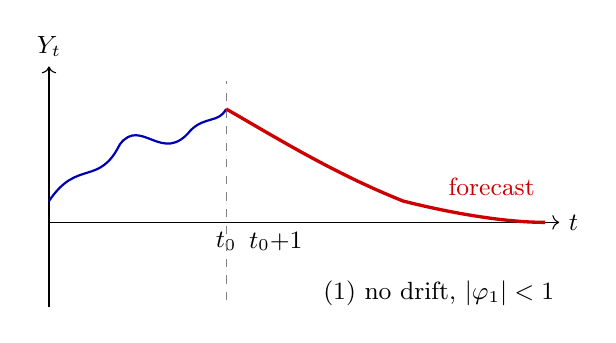
\begin{tikzpicture}[scale=0.9]
% Figure (1): AR(1) no drift, forecast decays to 0
\begin{scope}
  \draw[->] (0,0) -- (7.2,0) node[right,font=\small] {$t$};
  \draw[->] (0,-1.2) -- (0,2.2) node[above,font=\small] {$Y_t$};
  % axis labels
  \node[below,font=\small] at (2.5,0) {$t_0$};
  \node[below,font=\small] at (3.2,0) {$t_0{+}1$};
  \draw[dashed,gray] (2.5,-1.1) -- (2.5,2.0);
  % observed path (blue wiggly)
  \draw[blue!70!black, thick]
    (0,0.3) .. controls (0.4,0.9) and (0.7,0.5) ..
    (1.0,1.1) .. controls (1.3,1.5) and (1.6,0.8) ..
    (2.0,1.3) .. controls (2.2,1.5) and (2.4,1.4) ..
    (2.5,1.6);
  % forecast (red, decaying to 0)
  \draw[red!80!black, very thick]
    (2.5,1.6) .. controls (3.2,1.2) and (4.0,0.7) ..
    (5.0,0.3) .. controls (5.8,0.1) and (6.5,0.0) ..
    (7.0,0.0);
  % labels
  \node[right,font=\small,red!80!black] at (5.5,0.5) {forecast};
  \node[font=\small] at (5.5,-1.0) {(1) no drift, $|\varphi_1|<1$};
\end{scope}
\end{tikzpicture}
\hspace{1.5cm}
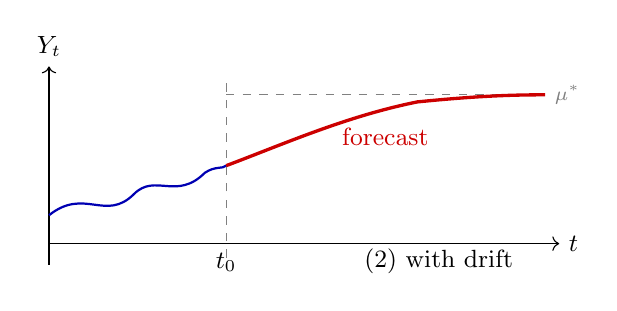
\begin{tikzpicture}[scale=0.9]
% Figure (2): AR(1) with drift, forecast rises to equilibrium
\begin{scope}
  \draw[->] (0,0) -- (7.2,0) node[right,font=\small] {$t$};
  \draw[->] (0,-0.3) -- (0,2.5) node[above,font=\small] {$Y_t$};
  \node[below,font=\small] at (2.5,0) {$t_0$};
  \draw[dashed,gray] (2.5,-0.2) -- (2.5,2.3);
  % equilibrium line
  \draw[gray,dashed] (2.5,2.1) -- (7.0,2.1)
    node[right,font=\scriptsize,gray] {$\mu^*$};
  % observed path (blue wiggly)
  \draw[blue!70!black, thick]
    (0,0.4) .. controls (0.5,0.8) and (0.8,0.3) ..
    (1.2,0.7) .. controls (1.5,1.0) and (1.8,0.6) ..
    (2.2,1.0) .. controls (2.35,1.1) and (2.45,1.05) ..
    (2.5,1.1);
  % forecast (red, rising to equilibrium)
  \draw[red!80!black, very thick]
    (2.5,1.1) .. controls (3.3,1.4) and (4.2,1.8) ..
    (5.2,2.0) .. controls (6.0,2.08) and (6.5,2.1) ..
    (7.0,2.1);
  \node[right,font=\small,red!80!black] at (4.0,1.5) {forecast};
  \node[font=\small] at (5.5,-0.25) {(2) with drift};
\end{scope}
\end{tikzpicture}
\end{center}

Notice what \eqref{eq:ar1_forecast} depends on: only $\varphi_0$,
$\varphi_1$, and $Y_{t_0}$. The noise parameter $\sigma$ does not appear.
The same forecast curve is consistent with an entire family of AR(1)
processes, indexed by $\sigma > 0$.

\subsection{Many processes, one forecast}

Fix $\varphi_0$ and $\varphi_1$ with $|\varphi_1|<1$, and let $\sigma$
vary. Each choice of $\sigma$ defines a different probability measure on
path space, yet all produce the same optimal point forecast. The forecast
curve does not determine the underlying process.

Figure~(1a) extends Figure~(1) by adding the bundle of sample paths
(green) consistent with the observed history and the AR(1) model for any
$\sigma>0$. The red line is the same MSE-optimal forecast regardless.
Figure~(1b) shows a more concentrated bundle, corresponding to a smaller
$\sigma$---the red forecast is identical.

\begin{center}
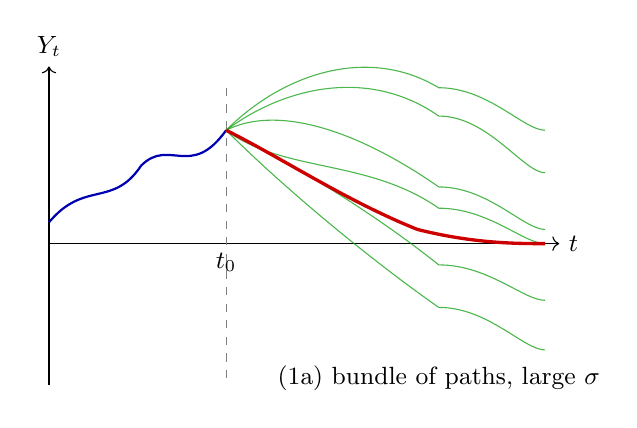
\begin{tikzpicture}[scale=0.9]
% Figure (1a): no drift + many green paths spreading out
\draw[->] (0,0) -- (7.2,0) node[right,font=\small] {$t$};
\draw[->] (0,-2.0) -- (0,2.5) node[above,font=\small] {$Y_t$};
\node[below,font=\small] at (2.5,0) {$t_0$};
\draw[dashed,gray] (2.5,-1.9) -- (2.5,2.3);
% several green future paths (spread wide)
\foreach \ys/\ca/\cb/\cc/\ye in {
  1.6/2.0/1.5/0.8/0.2,
  1.6/2.2/2.5/1.8/1.0,
  1.6/1.2/0.5/-0.3/-0.8,
  1.6/0.8/-0.2/-0.9/-1.5,
  1.6/2.4/2.8/2.2/1.6,
  1.6/1.0/1.2/0.5/0.0
}{
  \draw[green!60!black, opacity=0.7]
    (2.5,\ys) .. controls (3.3,\ca) and (4.5,\cb) ..
    (5.5,\cc) .. controls (6.2,\cc) and (6.7,\ye) .. (7.0,\ye);
}
% observed path blue
\draw[blue!70!black, thick]
  (0,0.3) .. controls (0.5,0.9) and (0.9,0.5) ..
  (1.3,1.1) .. controls (1.7,1.5) and (2.0,0.9) ..
  (2.5,1.6);
% red forecast
\draw[red!80!black, very thick]
  (2.5,1.6) .. controls (3.3,1.2) and (4.2,0.6) ..
  (5.2,0.2) .. controls (6.0,0.0) and (6.6,0.0) .. (7.0,0.0);
\node[font=\small] at (5.5,-1.9) {(1a) bundle of paths, large $\sigma$};
\end{tikzpicture}
\hspace{1.0cm}
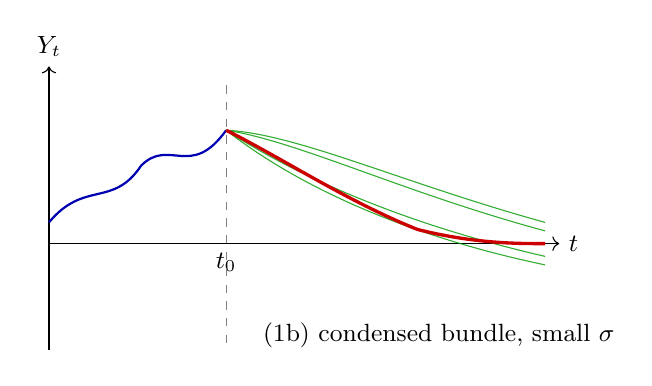
\begin{tikzpicture}[scale=0.9]
% Figure (1b): no drift + condensed green paths
\draw[->] (0,0) -- (7.2,0) node[right,font=\small] {$t$};
\draw[->] (0,-1.5) -- (0,2.5) node[above,font=\small] {$Y_t$};
\node[below,font=\small] at (2.5,0) {$t_0$};
\draw[dashed,gray] (2.5,-1.4) -- (2.5,2.3);
% condensed green paths - both above and below red
% red goes: (2.5,1.6) -> (3.5,1.2) -> (5.0,0.5) -> (7.0,0.0)
% above red
\draw[green!60!black, opacity=0.8]
  (2.5,1.6) .. controls (3.5,1.55) and (5.0,0.85) .. (7.0,0.30);
\draw[green!60!black, opacity=0.8]
  (2.5,1.6) .. controls (3.5,1.45) and (5.0,0.72) .. (7.0,0.18);
% below red
\draw[green!60!black, opacity=0.8]
  (2.5,1.6) .. controls (3.5,0.95) and (5.0,0.28) .. (7.0,-0.18);
\draw[green!60!black, opacity=0.8]
  (2.5,1.6) .. controls (3.5,0.82) and (5.0,0.12) .. (7.0,-0.30);
% observed path blue
\draw[blue!70!black, thick]
  (0,0.3) .. controls (0.5,0.9) and (0.9,0.5) ..
  (1.3,1.1) .. controls (1.7,1.5) and (2.0,0.9) ..
  (2.5,1.6);
% red forecast
\draw[red!80!black, very thick]
  (2.5,1.6) .. controls (3.3,1.2) and (4.2,0.6) ..
  (5.2,0.2) .. controls (6.0,0.0) and (6.6,0.0) .. (7.0,0.0);
\node[font=\small] at (5.5,-1.3) {(1b) condensed bundle, small $\sigma$};
\end{tikzpicture}
\end{center}

The red line is the same in both figures. This illustrates the
decoupling: $\sigma$ determines the width of the bundle but not the
forecast.

This is not a bug. For the purpose of minimising MSE of a point predictor,
$\sigma$ is simply irrelevant---it drops out of the first-order condition.
It becomes relevant only when we ask about prediction intervals, or about
the density of $Y_{t_0+h}$ rather than its expectation.

\subsection{Causal AR(1) and its MA($\infty$) representation}

An AR(1) process is called \textbf{causal} if it can be expressed as a
linear combination of present and past innovations only.
This holds if and only if $|\varphi_1| < 1$.
A causal AR(1) then has an MA($\infty$) representation:
\[
  Y_t = \frac{\varphi_0}{1-\varphi_1} + \sum_{k=0}^{\infty} \varphi_1^k \ve_{t-k}.
\]
The coefficient sequence $\{1, \varphi_1, \varphi_1^2, \ldots\}$ decays
geometrically. Any two AR(1) processes with the same $\varphi_0, \varphi_1$
but different $\sigma$ share this coefficient sequence; they differ only in
the scale of the driving noise.

\subsection{Known vs.\ estimated coefficients; the plug-in step}

The analysis above assumed $\varphi_0$ and $\varphi_1$ are known. In
practice they are estimated from data, and the plug-in principle is
applied: replace $\varphi_0, \varphi_1$ by $\hat\varphi_0, \hat\varphi_1$
in \eqref{eq:ar1_forecast}. This step is almost always performed without
comment in textbooks, and the resulting uncertainty in the forecast---from
estimating the coefficients---is typically ignored at the level of point
prediction.

Formally, the plug-in forecast is no longer optimal in the MSE sense for
the true unknown $\varphi_1$; it is optimal only if the estimates are
exact. The additional estimation variance contributes to the total forecast
error but is absorbed into the residual term.

\subsection{Optimality for multi-step forecasts}

A natural question is whether the recursive formula---use the one-step
forecast as a pseudo-observation, then apply the AR(1) recursion again---is
optimal for $h > 1$.

The answer is yes, under the assumption that the process is AR(1) with
known coefficients and the error is mean-zero. The $h$-step conditional
expectation $\E[Y_{t_0+h} \mid Y_0, \ldots, Y_{t_0}]$ equals
\eqref{eq:ar1_forecast}, and this conditional expectation is the MSE-optimal
predictor by the standard argument (it minimises
$\E[(Y_{t_0+h} - f(Y_0,\ldots,Y_{t_0}))^2]$ over all measurable $f$).

When coefficients are estimated via plug-in, the recursive formula is still
standard practice; its optimality in that setting requires a separate
argument which is often omitted in applied texts.

\subsection{Summary}

\begin{itemize}
\item A forecast curve determines the conditional mean, not the full
  distribution. Many AR(1) processes (differing in $\sigma$) share the same
  forecast.
\item $\sigma$ is invisible to point forecasting but essential for
  prediction intervals.
\item AR(1) is causal when $|\varphi_1|<1$, and causal AR(1) has an
  MA($\infty$) representation. This makes explicit why $\sigma$ decouples:
  it enters only as a scale on the driving noise, not in the coefficient
  sequence.
\item Plug-in of estimated coefficients is universally applied but
  introduces additional uncertainty that point-forecast theory does not
  account for.
\item Multi-step recursive forecasts are MSE-optimal when coefficients are
  known; the plug-in case is left implicit in most treatments.
\end{itemize}

%--------------------------------------------------------------------
\section{Conclusion}
%--------------------------------------------------------------------

This note is eclectic by design. Three threads that happened to cross
during the same week at work.

The cohort component recursion, under constant rates, is AR(1). Not an
approximation---the same equation. Equilibrium size is $I/r^O$, the fixed
point; convergence speed is $1-r^O$. The multi-group case is VAR(1). If
you are building a workforce or membership forecast on cohort dynamics,
the time-series toolkit applies directly.

Point forecasting in the i.i.d.\ setting: predictive MSE and estimation
MSE differ by exactly $\mathrm{Var}(Y)$, for every predictor. That gap
is irreducible. Best predictor and best estimator of $\E Y$ are the same
statistic; they just measure against different targets.

And the question that connects the two: the forecast curve does not
determine the underlying process. For AR(1), the same point forecast is
consistent with any $\sigma > 0$. Prediction and inference are related
but separate problems, and the plug-in step that bridges them is usually
performed without comment.

\end{document}
